\chapter{VaR and Credit Risk}\label{var-and-credit-risk}

VaR is an acronym of ‘Value at Risk’, and is a tool which is used by many firms and banks to establish the level of financial risk within its firm. The VaR is calculated for an investments of a company’s investments or perhaps for checking the riks levels of a portfolio managed by the wealth management branch of a bank or a boutique firm.


The risk taken on by an entity entering a contract with one (or more) counter-party having a relevant default
probability. As such, the counter-party might not respect its payment obligations.


\section{Value at Risk}\label{value-at-risk}

The value at risk (VaR) of a portfolio is a function of two parameters
(time horizon and confidence level) and it is usually involved when it
is important to know to a certain confidence level how
much will be the maximum loss in the next $N$ days. 

It can be interpreted as the loss level over \(N\) days that has a 
probability of only \((100 - X)\%\) of being exceeded.
Mathematically the VaR is the loss corresponding to the
\((100-X)\textrm{th}\) percentile of the distribution of the change in
the value of the portfolio over the next \(N\) days. 

For example, with \(N=1\) and \(X=95\), VaR is the fifth percentile of the distribution of
changes in the value of the portfolio over the next day (e.g. in Figure~\ref{fig:var_loss}
the graphical representation of the VaR assuming a normal
distribution for the changes of value.

\begin{figure}
\centering
  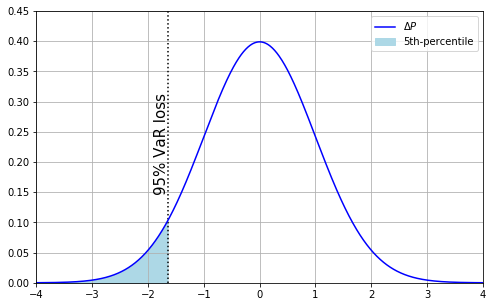
\includegraphics[width=0.6\linewidth]{figures/95_var.png}
  \caption{Example of 95\% VaR on the distribution of changes in the value.}
  \label{fig:var_loss}
\end{figure}
    
VaR is useful to summarize all the information about the risk of a
portfolio in one single number, but this can also be considered its main
limitation (as it implies too much simplification).

Concerning the time horizon parameter it is usually set to \(N=1\) since
it is not easy to estimate market variables over periods longer than one
day. To generalize the VaR estimate it is assumed:

\begin{equation}
\textrm{N-day VaR} = \textrm{1-day VaR}\times \sqrt{N}
\label{eq:var_horizon}
\end{equation}

This relation is true only if the changes of value of the portfolio over
the considered period of time have independent and identical normal
distributions with mean 0 (otherwise it is just an approximation).

\section{How to Estimate the VaR}\label{how-to-estimate-the-var}

Three are the methods that can be used to estimate the VaR.
In this Section they will be reviewed.

In the proposed examples historical series of Apple and Netflix will 
are used. Data is saved in \href{}{historical\_data.csv}.
It can be inspected as usual with \texttt{pandas}.
We will assume to have a portfolio made of 60\% of AAPL and 40\% NFLX stocks.

\begin{tcolorbox}[breakable, size=fbox, boxrule=1pt, pad at break*=1mm,colback=cellbackground, colframe=cellborder]
\begin{Verbatim}[commandchars=\\\{\}]
\PY{k+kn}{import} \PY{n+nn}{pandas} \PY{k}{as} \PY{n+nn}{pd}
\PY{k+kn}{import} \PY{n+nn}{numpy} \PY{k}{as} \PY{n+nn}{np}

\PY{n}{w} \PY{o}{=} \PY{n}{np}\PY{o}{.}\PY{n}{array}\PY{p}{(}\PY{p}{[}\PY{l+m+mf}{0.6}\PY{p}{,} \PY{l+m+mf}{0.4}\PY{p}{]}\PY{p}{)}
\PY{n}{df} \PY{o}{=} \PY{n}{pd}\PY{o}{.}\PY{n}{read\PYZus{}csv}\PY{p}{(}\PY{l+s+s2}{\PYZdq{}}\PY{l+s+s2}{quandl.csv}\PY{l+s+s2}{\PYZdq{}}\PY{p}{)}
\PY{n}{aapl} \PY{o}{=} \PY{n}{df}\PY{p}{[}\PY{n}{df}\PY{p}{[}\PY{l+s+s1}{\PYZsq{}}\PY{l+s+s1}{ticker}\PY{l+s+s1}{\PYZsq{}}\PY{p}{]}\PY{o}{==}\PY{l+s+s2}{\PYZdq{}}\PY{l+s+s2}{AAPL}\PY{l+s+s2}{\PYZdq{}}\PY{p}{]}\PY{o}{.}\PY{n}{copy}\PY{p}{(}\PY{p}{)}
\PY{n}{nlfx} \PY{o}{=} \PY{n}{df}\PY{p}{[}\PY{n}{df}\PY{p}{[}\PY{l+s+s1}{\PYZsq{}}\PY{l+s+s1}{ticker}\PY{l+s+s1}{\PYZsq{}}\PY{p}{]}\PY{o}{==}\PY{l+s+s2}{\PYZdq{}}\PY{l+s+s2}{NFLX}\PY{l+s+s2}{\PYZdq{}}\PY{p}{]}\PY{o}{.}\PY{n}{copy}\PY{p}{(}\PY{p}{)}
		
\PY{n}{aapl}\PY{p}{[}\PY{l+s+s1}{\PYZsq{}}\PY{l+s+s1}{rets}\PY{l+s+s1}{\PYZsq{}}\PY{p}{]} \PY{o}{=} \PY{n}{aapl}\PY{p}{[}\PY{l+s+s1}{\PYZsq{}}\PY{l+s+s1}{adj\PYZus{}close}\PY{l+s+s1}{\PYZsq{}}\PY{p}{]}\PY{o}{/}\PY{n}{aapl}\PY{p}{[}\PY{l+s+s1}{\PYZsq{}}\PY{l+s+s1}{adj\PYZus{}close}\PY{l+s+s1}{\PYZsq{}}\PY{p}{]}\PY{o}{.}\PY{n}{shift}\PY{p}{(}\PY{l+m+mi}{1}\PY{p}{)} \PY{o}{\PYZhy{}} \PY{l+m+mi}{1}
\PY{n}{nflx}\PY{p}{[}\PY{l+s+s1}{\PYZsq{}}\PY{l+s+s1}{rets}\PY{l+s+s1}{\PYZsq{}}\PY{p}{]} \PY{o}{=} \PY{n}{nflx}\PY{p}{[}\PY{l+s+s1}{\PYZsq{}}\PY{l+s+s1}{adj\PYZus{}close}\PY{l+s+s1}{\PYZsq{}}\PY{p}{]}\PY{o}{/}\PY{n}{nflx}\PY{p}{[}\PY{l+s+s1}{\PYZsq{}}\PY{l+s+s1}{adj\PYZus{}close}\PY{l+s+s1}{\PYZsq{}}\PY{p}{]}\PY{o}{.}\PY{n}{shift}\PY{p}{(}\PY{l+m+mi}{1}\PY{p}{)} \PY{o}{\PYZhy{}} \PY{l+m+mi}{1}

\PY{n+nb}{print} \PY{p}{(}\PY{n}{aapl}\PY{o}{.}\PY{n}{head}\PY{p}{(}\PY{p}{)}\PY{p}{)}

            date ticker adj\_close      rets
4201  2018-03-27   AAPL    168.340       NaN
4202  2018-03-26   AAPL    172.770  0.026316
4203  2018-03-23   AAPL    164.940 -0.045320
4204  2018-03-22   AAPL    168.845  0.023675
4205  2018-03-21   AAPL    171.270  0.014362
\end{Verbatim}
\end{tcolorbox}

\subsection{Historical Simulation}\label{historical-simulation}

In order to estimate the VaR from an historical series, we need to
collect the market variables affecting the portfolio over the last \(N\)
days (with \(N\) quite large).

The variation over each day in our time interval will provide different
scenarios to be applied to today's market simulation so that for each of
them we need to compute the variation in the portfolio value
(\(\Delta P\)). 

Given the distribution of the simulated scenarios the VaR estimate 
will be its (100 - X)\% percentile. 

Of course such historical simulation relies on the assumption that past
behaviors are indicative of what might happen in the future, that's why it 
is important that out historical series was as large as possible.

As an example imagine a portfolio \(P\) whose value depends only on two market
variables (\(x_1(t) , x_2(t)\)). From the historical series of these
variables we can determine various \emph{simulated} portfolio
values:

\[P_i(t_n+1) = P\Big(x_1(t_n)\cfrac{(x_1(t_i)-x_1(t_{i-1}))}{x_1(t_{i-1})}, x_2(t_n)\cfrac{(x_2(t_i)-x_2(t_{i-1}))}{x_2(t_{i-1})}\Big)\]

Essentially re-scaling the market variables according to the variation
between day \(i\) and \(i-1\) we can draw a distribution of the possible
changes in the portfolio value \(P_i\) and then compute the VaR taking
the appropriate percentile.

Using the historical series seen above the procedure can be outlined as follows. Figure~\ref{fig:hist_var} shows the resulting VaR.

\begin{tcolorbox}[breakable, size=fbox, boxrule=1pt, pad at break*=1mm,colback=cellbackground, colframe=cellborder]
\begin{Verbatim}[commandchars=\\\{\}]
\PY{c+c1}{\PYZsh{} historical VaR}
\PY{k+kn}{import} \PY{n+nn}{numpy} \PY{k}{as} \PY{n+nn}{np}
				
\PY{n}{rets} \PY{o}{=} \PY{p}{[}\PY{p}{]}
\PY{k}{for} \PY{n}{i} \PY{o+ow}{in} \PY{n+nb}{range}\PY{p}{(}\PY{l+m+mi}{1}\PY{p}{,} \PY{n+nb}{len}\PY{p}{(}\PY{n}{aapl}\PY{p}{)}\PY{p}{)}\PY{p}{:}
    \PY{n}{rets}\PY{o}{.}\PY{n}{append}\PY{p}{(}\PY{n}{w}\PY{p}{[}\PY{l+m+mi}{0}\PY{p}{]}\PY{o}{*}\PY{n}{aapl}\PY{o}{.}\PY{n}{iloc}\PY{p}{[}\PY{n}{i}\PY{p}{]}\PY{p}{[}\PY{l+s+s1}{\PYZsq{}}\PY{l+s+s1}{rets}\PY{l+s+s1}{\PYZsq{}}\PY{p}{]} \PY{o}{+} \PY{n}{w}\PY{p}{[}\PY{l+m+mi}{1}\PY{p}{]}\PY{o}{*}\PY{n}{nflx}\PY{o}{.}\PY{n}{loc}\PY{p}{[}\PY{n}{i}\PY{p}{]}\PY{p}{[}\PY{l+s+s1}{\PYZsq{}}\PY{l+s+s1}{rets}\PY{l+s+s1}{\PYZsq{}}\PY{p}{]}\PY{p}{)}
		
\PY{n}{price} \PY{o}{=} \PY{p}{[}\PY{n}{aapl}\PY{o}{.}\PY{n}{iloc}\PY{p}{[}\PY{o}{\PYZhy{}}\PY{l+m+mi}{1}\PY{p}{]}\PY{p}{[}\PY{l+s+s1}{\PYZsq{}}\PY{l+s+s1}{adj\PYZus{}close}\PY{l+s+s1}{\PYZsq{}}\PY{p}{]}\PY{p}{,} \PY{n}{nflx}\PY{o}{.}\PY{n}{iloc}\PY{p}{[}\PY{o}{\PYZhy{}}\PY{l+m+mi}{1}\PY{p}{]}\PY{p}{[}\PY{l+s+s1}{\PYZsq{}}\PY{l+s+s1}{adj\PYZus{}close}\PY{l+s+s1}{\PYZsq{}}\PY{p}{]}\PY{p}{]}
		
\PY{n}{portfolio\PYZus{}price} \PY{o}{=} \PY{n}{w}\PY{o}{.}\PY{n}{dot}\PY{p}{(}\PY{n}{price}\PY{p}{)}
		
\PY{n}{hist\PYZus{}var} \PY{o}{=} \PY{n}{portfolio\PYZus{}price}\PY{o}{*}\PY{n}{np}\PY{o}{.}\PY{n}{percentile}\PY{p}{(}\PY{n}{rets}\PY{p}{,} \PY{l+m+mi}{1}\PY{p}{)}
\PY{n+nb}{print} \PY{p}{(}\PY{l+s+s1}{\PYZsq{}}\PY{l+s+s1}{Historical VAR is }\PY{l+s+si}{\PYZob{}:.3f\PYZcb{}}\PY{l+s+s1}{\PYZsq{}}\PY{o}{.}\PY{n}{format}\PY{p}{(}\PY{n}{hist\PYZus{}var}\PY{p}{)}\PY{p}{)}

Historical VAR is -2.412
\end{Verbatim}
\end{tcolorbox}

\begin{figure}
	\centering
	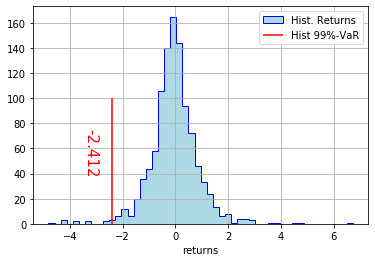
\includegraphics[width=0.7\textwidth]{figures/Untitled_0_1.png}
	\caption{Distribution of the changes of values estimated from historical data. The red line shows the 99\% VaR.}
	\label{fig:hist_var}
\end{figure}

\subsection{Model Approach}\label{model-approach}

Our portfolio \(P\) consists of different amounts \(w_i\)
invested on two assets. If with \(\Delta x_i\) we denote the daily
return of the $i$th asset the change in the value of the portfolio can be
expressed as:

\[\Delta P = \sum_{i=1}^n w_i \Delta x_i\]

If we then assume that the asset variations are normally distributed
with mean 0 (in this approach is typical to assume the expected change
in a market variable over the considered period zero), \(\Delta P\) will
be normally distributed (as a sum of normal distribution) with zero
mean.

To estimate the VaR we just need to compute the standard deviation of
\(\Delta P\). In the general case with many different assets we define
\(\sigma_i\) the daily volatility of the $i$th asset and with
\(\rho_{ij}\) the correlation coefficient between the assets $i$ and $j$.
The variance of \(\Delta P\) can then be expressed as:

\begin{align*}\sigma^2_P & = \sum_{i=1}^{n}\sum_{j=1}^{n}\rho_{ij}w_i w_j \sigma_i \sigma_j \\
& = \sum_{i=1}^{n} w_i^2 \sigma_i^2 + 2 \sum_{i=1}^{n}\sum_{j<i}^{n}\rho_{ij}w_i w_j \sigma_i \sigma_j 
\end{align*}

As in the previous case if we are interested in a longer time horizon we
can use Eq.~\ref{eq:var_horizon}.

Once we have the variance of \(\Delta P\) it is easy to determine the appropriate percentile using the equations described in Appendix~\ref{transformation-to-standard-normal}.


\subsection{Monte Carlo Simulation}\label{monte-carlo-simulation}

A very useful alternative to the previous approaches is using a Monte
Carlo simulation to generate the probability distribution for the
\(\Delta P\) distribution. 

Imagine we need to compute the 1-day VaR for our example portfolio
the simulation can be done either generating random returns from a distribution with mean and standard deviation obtained from the historical data of each stock, or by simulating the evolution 
of all the portfolio market variables in one day.

Let's start from the first case, computing mean and standard deviation of each historical data-set. We will then throw various simulated returns from a multivariate Gaussian with such means and variances. 
One useful aspect of this method is that in principal other distribution could be used instead of a Gaussian.
Once we have the distribution of returns the VaR can be computed as usual, the example distribution is shown in Fig.~\ref{fig:mc1_var}.

\begin{tcolorbox}[breakable, size=fbox, boxrule=1pt, pad at break*=1mm,colback=cellbackground, colframe=cellborder]
\begin{Verbatim}[commandchars=\\\{\}]
\PY{c+c1}{\PYZsh{} MC simulated VaR 1}
\PY{k+kn}{from} \PY{n+nn}{scipy}\PY{n+nn}{.}\PY{n+nn}{stats} \PY{k}{import} \PY{n}{norm}		
\PY{k+kn}{from} \PY{n+nn}{scipy}\PY{n+nn}{.}\PY{n+nn}{stats} \PY{k}{import} \PY{n}{multivariate\PYZus{}normal}
		
\PY{n}{mean} \PY{o}{=} \PY{p}{[}\PY{n}{np}\PY{o}{.}\PY{n}{mean}\PY{p}{(}\PY{n}{aapl}\PY{p}{[}\PY{l+s+s1}{\PYZsq{}}\PY{l+s+s1}{rets}\PY{l+s+s1}{\PYZsq{}}\PY{p}{]}\PY{p}{)}\PY{p}{,} \PY{n}{np}\PY{o}{.}\PY{n}{mean}\PY{p}{(}\PY{n}{nflx}\PY{p}{[}\PY{l+s+s1}{\PYZsq{}}\PY{l+s+s1}{rets}\PY{l+s+s1}{\PYZsq{}}\PY{p}{]}\PY{p}{)}\PY{p}{]}
\PY{n}{std} \PY{o}{=} \PY{p}{[}\PY{n}{np}\PY{o}{.}\PY{n}{std}\PY{p}{(}\PY{n}{aapl}\PY{p}{[}\PY{l+s+s1}{\PYZsq{}}\PY{l+s+s1}{rets}\PY{l+s+s1}{\PYZsq{}}\PY{p}{]}\PY{p}{)}\PY{p}{,} \PY{n}{np}\PY{o}{.}\PY{n}{std}\PY{p}{(}\PY{n}{nflx}\PY{p}{[}\PY{l+s+s1}{\PYZsq{}}\PY{l+s+s1}{rets}\PY{l+s+s1}{\PYZsq{}}\PY{p}{]}\PY{p}{)}\PY{p}{]}
		
\PY{n}{mvnorm} \PY{o}{=} \PY{n}{multivariate\PYZus{}normal}\PY{p}{(}\PY{n}{mean}\PY{o}{=}\PY{n}{mean}\PY{p}{,} \PY{n}{cov}\PY{o}{=}\PY{p}{[}\PY{p}{[}\PY{n}{std}\PY{p}{[}\PY{l+m+mi}{0}\PY{p}{]}\PY{o}{*}\PY{o}{*}\PY{l+m+mi}{2}\PY{p}{,} \PY{l+m+mi}{0}\PY{p}{]}\PY{p}{,}
                                             \PY{p}{[}\PY{l+m+mi}{0}\PY{p}{,} \PY{n}{std}\PY{p}{[}\PY{l+m+mi}{1}\PY{p}{]}\PY{o}{*}\PY{o}{*}\PY{l+m+mi}{2}\PY{p}{]}\PY{p}{]}\PY{p}{)}
\PY{n}{n\PYZus{}sims} \PY{o}{=} \PY{l+m+mi}{100000}
\PY{n}{sim\PYZus{}returns} \PY{o}{=} \PY{n}{mvnorm}\PY{o}{.}\PY{n}{rvs}\PY{p}{(}\PY{n}{n\PYZus{}sims}\PY{p}{)}
\PY{n}{p\PYZus{}returns} \PY{o}{=} \PY{p}{[}\PY{n}{w}\PY{o}{.}\PY{n}{dot}\PY{p}{(}\PY{n}{s}\PY{p}{)} \PY{k}{for} \PY{n}{s} \PY{o+ow}{in} \PY{n}{sim\PYZus{}returns}\PY{p}{]}
\PY{n}{mc\PYZus{}var} \PY{o}{=} \PY{n}{portfolio\PYZus{}price} \PY{o}{*} \PY{n}{np}\PY{o}{.}\PY{n}{percentile}\PY{p}{(}\PY{n}{p\PYZus{}returns}\PY{p}{,} \PY{l+m+mi}{1}\PY{p}{)}
\PY{n+nb}{print}\PY{p}{(}\PY{l+s+s1}{\PYZsq{}}\PY{l+s+s1}{Simulated VAR is }\PY{l+s+si}{\PYZob{}\PYZcb{}}\PY{l+s+s1}{\PYZsq{}}\PY{p}{,} \PY{n}{mc\PYZus{}var}\PY{p}{)}

Simulated VAR is \{\} -2.114679008811982
\end{Verbatim}
\end{tcolorbox}

\begin{figure}[htb]
	\centering
	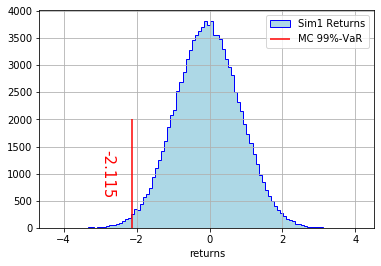
\includegraphics[width=0.7\textwidth]{figures/Untitled_2_1.png}
	\caption{Distribution of the changes of values estimated from simulated data. The red line shows the 99\% VaR.}
	\label{fig:mc1_var}
\end{figure}

This result can be compared with the VaR estimated with a simulation of the daily evolution of the stock price. We will use the log-normal evolution described in Section~\ref{derivation-of-log-normal-stochastic-differential-equation} where $\mu$ and $\sigma@$ are the mean and variance estimated from the historical series. Figure~\ref{fig:mc2_var} shows the resulting distribution of the returns.

\begin{tcolorbox}[breakable, size=fbox, boxrule=1pt, pad at break*=1mm,colback=cellbackground, colframe=cellborder]
\begin{Verbatim}[commandchars=\\\{\}]
\PY{k+kn}{from} \PY{n+nn}{numpy} \PY{k}{import} \PY{n}{exp}\PY{p}{,} \PY{n}{sqrt}
		
\PY{n}{T} \PY{o}{=} \PY{l+m+mi}{1}
\PY{n}{trials} \PY{o}{=} \PY{l+m+mi}{100000}
\PY{n}{dP} \PY{o}{=} \PY{p}{[}\PY{p}{]}
		
\PY{k}{for} \PY{n}{\PYZus{}} \PY{o+ow}{in} \PY{n+nb}{range}\PY{p}{(}\PY{n}{trials}\PY{p}{)}\PY{p}{:}
    \PY{n}{s} \PY{o}{=} \PY{l+m+mi}{0}
    \PY{k}{for} \PY{n}{i} \PY{o+ow}{in} \PY{n+nb}{range}\PY{p}{(}\PY{l+m+mi}{2}\PY{p}{)}\PY{p}{:}
        \PY{n}{s} \PY{o}{+}\PY{o}{=} \PY{n}{w}\PY{p}{[}\PY{n}{i}\PY{p}{]} \PY{o}{*} \PY{n}{price}\PY{p}{[}\PY{n}{i}\PY{p}{]} \PY{o}{*} \PY{n}{exp}\PY{p}{(}\PY{p}{(}\PY{n}{mean}\PY{p}{[}\PY{n}{i}\PY{p}{]} \PY{o}{\PYZhy{}} \PY{l+m+mf}{0.5} \PY{o}{*} \PY{n}{std}\PY{p}{[}\PY{n}{i}\PY{p}{]}\PY{o}{*}\PY{o}{*}\PY{l+m+mi}{2}\PY{p}{)} \PY{o}{*} \PY{n}{T} \PY{o}{+} 
                                   \PY{n}{std}\PY{p}{[}\PY{n}{i}\PY{p}{]} \PY{o}{*} \PY{n}{sqrt}\PY{p}{(}\PY{n}{T}\PY{p}{)} \PY{o}{*} \PY{n}{normal}\PY{p}{(}\PY{p}{)}\PY{p}{)}
    \PY{n}{dP}\PY{o}{.}\PY{n}{append}\PY{p}{(}\PY{n}{portfolio\PYZus{}price} \PY{o}{\PYZhy{}} \PY{n}{s}\PY{p}{)}
		
\PY{n}{mc\PYZus{}var2} \PY{o}{=} \PY{n}{np}\PY{o}{.}\PY{n}{percentile}\PY{p}{(}\PY{n}{dP}\PY{p}{,} \PY{l+m+mi}{1}\PY{p}{)}
\PY{n+nb}{print}\PY{p}{(}\PY{l+s+s1}{\PYZsq{}}\PY{l+s+s1}{Simulated VAR is }\PY{l+s+si}{\PYZob{}\PYZcb{}}\PY{l+s+s1}{\PYZsq{}}\PY{p}{,} \PY{n}{mc\PYZus{}var2}\PY{p}{)}

Simulated VAR is \{\} -1.9213098361249987
\end{Verbatim}
\end{tcolorbox}

\begin{figure}[htb]
	\centering
	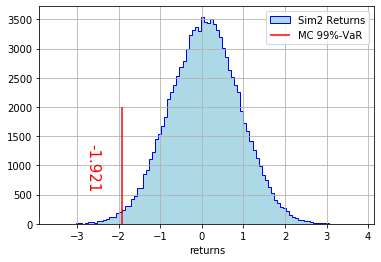
\includegraphics[width=0.7\textwidth]{figures/Untitled_3_1.png}
	\caption{Distribution of the changes of values estimated from simulation of the evolution of the stock prices. The red line shows the 99\% VaR.}
	\label{fig:mc2_var}
\end{figure}


\subsection{Stress and Back Testing}\label{stress-testing-and-back-testing}

In addition to calculating the value at risk of a portfolio, it could be useful to 
check how it would behave under the most extreme moves seen in the last years.

This kind of test is called \emph{stress test} and it is done by extracting from the historical series, particular days with exceptional large variation of our market variables, im order to check
how the portfolio moves.
 
The idea is to take into account extreme events that can more frequently in reality 
than in a simulation where Gaussian tails are assumed hence are quite hard to simulate
(e.g. a 5-standard deviation move should happen once every 7000 years
but in practice can be observed twice over 10 years).

How can we compute how likely is a $n\sigma$ event (assuming Gaussian distribution) ?
The probability of such a daily event is given by 1 over the total probability of having an 
event with a probability of $\pm n\sigma$ or more (the 252 factor comes to the number of working days per year).

\begin{tcolorbox}[breakable, size=fbox, boxrule=1pt, pad at break*=1mm,colback=cellbackground, colframe=cellborder]
\begin{Verbatim}[commandchars=\\\{\}]
\PY{k+kn}{from} \PY{n+nn}{scipy}\PY{n+nn}{.}\PY{n+nn}{stats} \PY{k}{import} \PY{n}{norm}

\PY{n}{prob} \PY{o}{=} \PY{n}{norm}\PY{o}{.}\PY{n}{cdf}\PY{p}{(}\PY{o}{\PYZhy{}}\PY{l+m+mi}{5}\PY{p}{)} \PY{o}{*} \PY{l+m+mi}{2} \PY{c+c1}{\PYZsh{} e.g. consider +\PYZhy{} 5sigma movements}
\PY{n}{nyears} \PY{o}{=} \PY{l+m+mi}{1}\PY{o}{/}\PY{n}{prob}\PY{o}{/}\PY{l+m+mi}{252}
\PY{n+nb}{print} \PY{p}{(}\PY{n}{nyears}\PY{p}{)}

6921.737673091067
    \end{Verbatim}
\end{tcolorbox}

Another important check that could be done is the so-called \emph{back testing}
which consists of checking how well the VaR estimate would have
performed in the past. Basically it has to be tested how often the daily
loss exceeded the N-days X\% VaR just computed. If it happens on about
(100-X)\% of the times we can be confident that our estimate is correct.

\section{Credit VaR}\label{credit-var-cr-var}

%exposure at any given future time is the
%larger between zero and the market value of the portfolio of derivative
%positions with a counterparty that would be lost if the counterparty
%were to default with zero recovery at that time.

Credit VaR is defined in the usual way Value at Risk measures are defined (i.e. as percentile of a loss).
In this case we are concerned with the default risk associated to one or
multiple counter-parties in a specific portfolio, and it is defined on
the overall exposure to all the counter-parties involved.

The exposure Ex at the default date is defined as:

\[ \textrm{Ex} = (\sum \Pi(\tau, T))^{+}\]

where \(\Pi(\tau,T)\) represents the discounted cash flows at the
default date \(\tau\); the corresponding loss is then given by:

\[L_{\tau, \hat{T}, T} = (1 - R) \cdot \textrm{Ex}(\tau)\]

where \(\hat{T}\) is the risk horizon and \(L\) is non-zero only in
scenarios of early default of the counter-party. Given the above
definitions we can express the Cr-VaR as the q-quantile of
\(L_{\tau, \hat{T}, T}\).

In this case the horizon is usually one year and the standard percentile is the 99.9th, so it returns the loss that is exceeded only in 1 case out of 1000. 

Cr-Var is actually either the difference of the percentile from the mean,
or the percentile itself. There is more than one possible definition.


%Consider your portfolio has a call option on equity with a final maturity of two years. To get the Credit-Var, roughly, you simulate the underlying equity up to one year, and obtain a number of scenarios for the underlying equity in one year. Also, you need to simulate the default scenarios up to one year, to know in each scenario whether the counter-parties have defaulted or not. 
%
%And then in each scenario at one year, if the counter-party
%has defaulted there will be a recovery value and all else will be lost.
%Otherwise, we price the call option over the remaining year using for
%example a Black Scholes formula. But this price is like taking the
%expected value of the call option payoff in two years, conditional on
%each scenario for the underlying equity in one year. Because this is
%pricing, this expected value will be taken under the pricing measure Q,
%not P. This gives the Black Scholes formula if the underlying equity
%follows a geometric brownian motion under Q.

\subsection{Credit Var and MC Simulation}

Credit VaR can be calculated through a simulation of the basic financial
variables underlying the portfolio up to the risk horizon. 
The simulation also includes the default of the counter-parties. 

At the risk horizon, the portfolio is priced in every simulated scenario of the basic financial variables, including defaults, obtaining a number of scenarios for the portfolio value at the risk horizon.

It is then straightforward to derive the Credit VaR from the distribution of the losses.

\subsection{Credit VaR and One Factor Copula Model}
Consider a portfolio made of similar assets. As an approximation assume that the probability of default is the same for each counter-party and that the correlation between each pair is the same and equal to $\rho$. If we use the One Factor Copula model to describe the default correlations, Eq.~\ref{eq:one_factor_model}

\[
\mathbb{P}(T|M) = \Phi\Big(\cfrac{\Phi^{-1}[Q(T)]-M\sqrt{\rho}}{\sqrt{1-\rho}}\Big)
\]
gives us the percentage of defaults by time $T$ as a function of $M$. 
Indeed if you a have $n$ counter-parties with the same default probability $DP(T)$ the percentage of defaults at time $T$ is $DP$ itself ($\textrm{\% of defaults} = \textrm{n defaults}/n = n\cdot DP/n$).

In the previous equation $\Phi$ is the cumulative distribution function of the standard normal.
Since $M$ is distributed according to a standard normal we can be $X\%$ certain that its value will be \emph{greater} than $\Phi^{-1}(1-X)=-\Phi^{-1}(X)$, where the last equality holds due to the symmetry of the Gaussian distribution (see Figure~\ref{fig:certain_for_X}).

\begin{figure}[htb]
	\centering
	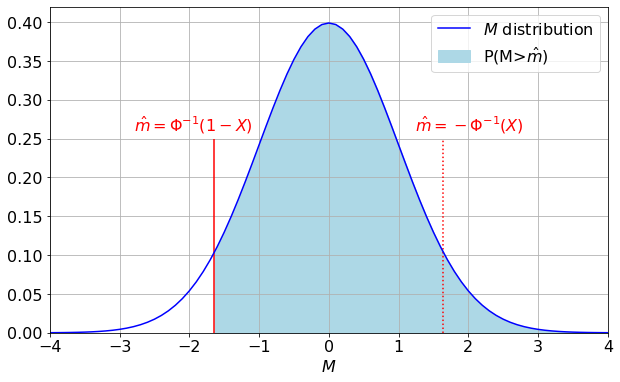
\includegraphics[width=0.7\textwidth]{figures/certain_for_X.png}
	\caption{$X\%$ probability to get an higher value a threshold for a normally distributed random variable.}
	\label{fig:certain_for_X}
\end{figure} 
But in the probability of default formula appears $-M$, therefore we are $X\%$ certain that the percentage of losses over $T$ years on a large portfolio will be \emph{less} than $V(X,T)$ where
\[
V(X,T)=\Phi\Big(\cfrac{\Phi^{-1}[Q(T)]+\Phi^{-1}(X)\sqrt{\rho}}{\sqrt{1-\rho}}\Big)
\]
When $X\%$ confidence level is used and the time horizon is $T$, a rough estimate of the Credit VaR is therefore $L(1-R)V(X,T)$, where $L$ is the size of the portfolio and $R$ is the recovery rate.

Suppose that a bank has a total of \euro{100} million of retail exposures. The 1-year probability of default averages to 2\% and the recovery rate averages to 60\%. The copula correlation parameter is estimated as 0.1.


\begin{tcolorbox}[breakable, size=fbox, boxrule=1pt, pad at break*=1mm,colback=cellbackground, colframe=cellborder]
\begin{Verbatim}[commandchars=\\\{\}]
\PY{k+kn}{from} \PY{n+nn}{scipy}\PY{n+nn}{.}\PY{n+nn}{stats} \PY{k}{import} \PY{n}{norm}
\PY{k+kn}{from} \PY{n+nn}{math} \PY{k}{import} \PY{n}{sqrt}
		
\PY{n}{X} \PY{o}{=} \PY{l+m+mf}{0.999}
\PY{n}{rho} \PY{o}{=} \PY{l+m+mf}{0.1}
\PY{n}{R} \PY{o}{=} \PY{l+m+mf}{0.6}
\PY{n}{DP} \PY{o}{=} \PY{l+m+mf}{0.02}
\PY{n}{exposure} \PY{o}{=} \PY{l+m+mf}{100e6}
		
\PY{n}{num} \PY{o}{=} \PY{n}{norm}\PY{o}{.}\PY{n}{ppf}\PY{p}{(}\PY{n}{DP}\PY{p}{)} \PY{o}{+} \PY{n}{sqrt}\PY{p}{(}\PY{n}{rho}\PY{p}{)}\PY{o}{*}\PY{n}{norm}\PY{o}{.}\PY{n}{ppf}\PY{p}{(}\PY{n}{X}\PY{p}{)}
\PY{n}{den} \PY{o}{=} \PY{n}{sqrt}\PY{p}{(}\PY{l+m+mi}{1}\PY{o}{\PYZhy{}}\PY{n}{rho}\PY{p}{)}
\PY{n}{V} \PY{o}{=} \PY{n}{norm}\PY{o}{.}\PY{n}{cdf}\PY{p}{(}\PY{n}{num}\PY{o}{/}\PY{n}{den}\PY{p}{)}
		
\PY{n}{cr\PYZus{}var} \PY{o}{=} \PY{n}{exposure}\PY{o}{*}\PY{n}{V}\PY{o}{*}\PY{p}{(}\PY{l+m+mi}{1}\PY{o}{\PYZhy{}}\PY{n}{R}\PY{p}{)}
\PY{n+nb}{print} \PY{p}{(}\PY{l+s+s2}{\PYZdq{}}\PY{l+s+s2}{Cr\PYZhy{}VaR: }\PY{l+s+si}{\PYZob{}:.0f\PYZcb{}}\PY{l+s+s2}{\PYZdq{}}\PY{o}{.}\PY{n}{format}\PY{p}{(}\PY{n+nb}{round}\PY{p}{(}\PY{n}{cr\PYZus{}var}\PY{p}{,} \PY{o}{\PYZhy{}}\PY{l+m+mi}{4}\PY{p}{)}\PY{p}{)}\PY{p}{)}

Cr-VaR: 5130000
\end{Verbatim}
\end{tcolorbox}
The 1-year 99.9\% Credit VaR is therefore \euro{5.13} million.

\subsection{CreditMetrics}
Another popular approach to compute Credti VaR is CreditMetrics. It involves estimating a probability distribution of credit losses by carrying out Monte Carlo simulations of the credit rating changes of all counter-parties.

Imagine we would like to determine the probability distribution of losses over 1-year period. On each simulation, the credit rating changes and default of each counter-parties is computed. The portfolio value is than computed to determine the eventual losses. 

As an example consider Table~\ref{tab:credit_ratings}, it shows the percentage probability of a bond moving from one category to another during a 1-year period.

\begin{table}[htb]
	\centering
	\begin{tabular}{|l|c|c|c|c|c|c|c|c|}
	\hline
	Initial rating & AAA & AA & A & BBB & BB & B & CCC & default \\
	\hline
	\hline
	AAA & 90.81 & 8.33 & 0.68 & 0.06 & 0.08 & 0.02 & 0.01& 0.01 \\ 
	\hline
	AA & 0.70 & 90.65 & 7.79 & 0.64 & 0.06 & 0.13 & 0.02 & 0.01 \\ 
	\hline
	A & 0.09 & 2.27 & 91.05 & 5.52 & 0.74 & 0.26 & 0.01 & 0.06 \\ 
	\hline
	BBB & 0.02 & 0.33 & 5.95 & 85.93 & 5.30 & 1.17 & 1.12 & 0.18 \\
	\hline
	BB & 0.03 & 0.14 & 0.67 & 7.73 & 80.53 & 8.84 & 1.00 & 1.06 \\
	\hline
	B & 0.01 & 0.11 & 0.24 & 0.43 & 6.48 & 83.46 & 4.07 & 5.20 \\
	\hline
	CCC & 0.21 & 0 & 0.22 & 1.30 & 2.38 & 11.24 & 64.86 & 19.79 \\		
	\hline
\end{tabular}
\caption{Example of table with transition probabilities (in percent) between different credit rating categories.}
\label{tab:credit_ratings}
\end{table}

Clearly credit rate changes cannot be assumed independent, hence a copula approach can be implemented also here.
As an example suppose to simulate rating change of a portfolio of 9 bonds with various ratings over 1-year period. The correlation between them is 0.2.

\begin{tcolorbox}[breakable, size=fbox, boxrule=1pt, pad at break*=1mm,colback=cellbackground, colframe=cellborder]
\begin{Verbatim}[commandchars=\\\{\}]
\PY{k+kn}{from} \PY{n+nn}{scipy}\PY{n+nn}{.}\PY{n+nn}{stats} \PY{k}{import} \PY{n}{multivariate\PYZus{}normal}\PY{p}{,} \PY{n}{norm}
\PY{k+kn}{import} \PY{n+nn}{numpy}
		
\PY{c+c1}{\PYZsh{} AAA, AA, A, BBB, BB, B, CCC, Def}
\PY{n}{table} \PY{o}{=} \PY{p}{[}\PY{p}{[}\PY{l+m+mf}{90.81}\PY{p}{,} \PY{l+m+mf}{8.33}\PY{p}{,} \PY{l+m+mf}{0.68}\PY{p}{,} \PY{l+m+mf}{0.06}\PY{p}{,} \PY{l+m+mf}{0.08}\PY{p}{,} \PY{l+m+mf}{0.02}\PY{p}{,} \PY{l+m+mf}{0.01}\PY{p}{,} \PY{l+m+mf}{0.01}\PY{p}{]}\PY{p}{,}
\PY{p}{[}\PY{l+m+mf}{0.70}\PY{p}{,} \PY{l+m+mf}{90.65}\PY{p}{,} \PY{l+m+mf}{7.79}\PY{p}{,} \PY{l+m+mf}{0.64}\PY{p}{,} \PY{l+m+mf}{0.06}\PY{p}{,} \PY{l+m+mf}{0.13}\PY{p}{,} \PY{l+m+mf}{0.02}\PY{p}{,} \PY{l+m+mf}{0.01}\PY{p}{]}\PY{p}{,}
\PY{p}{[}\PY{l+m+mf}{0.09}\PY{p}{,} \PY{l+m+mf}{2.27}\PY{p}{,} \PY{l+m+mf}{91.05}\PY{p}{,} \PY{l+m+mf}{5.52}\PY{p}{,} \PY{l+m+mf}{0.74}\PY{p}{,} \PY{l+m+mf}{0.26}\PY{p}{,} \PY{l+m+mf}{0.01}\PY{p}{,} \PY{l+m+mf}{0.06}\PY{p}{]}\PY{p}{,}
\PY{p}{[}\PY{l+m+mf}{0.02}\PY{p}{,} \PY{l+m+mf}{0.33}\PY{p}{,} \PY{l+m+mf}{5.95}\PY{p}{,} \PY{l+m+mf}{85.93}\PY{p}{,} \PY{l+m+mf}{5.30}\PY{p}{,} \PY{l+m+mf}{1.17}\PY{p}{,} \PY{l+m+mf}{1.12}\PY{p}{,} \PY{l+m+mf}{0.18}\PY{p}{]}\PY{p}{,}
\PY{p}{[}\PY{l+m+mf}{0.03}\PY{p}{,} \PY{l+m+mf}{0.14}\PY{p}{,} \PY{l+m+mf}{0.67}\PY{p}{,} \PY{l+m+mf}{7.73}\PY{p}{,} \PY{l+m+mf}{80.53}\PY{p}{,} \PY{l+m+mf}{8.84}\PY{p}{,} \PY{l+m+mf}{1.00}\PY{p}{,} \PY{l+m+mf}{1.06}\PY{p}{]}\PY{p}{,}
\PY{p}{[}\PY{l+m+mf}{0.01}\PY{p}{,} \PY{l+m+mf}{0.11}\PY{p}{,} \PY{l+m+mf}{0.24}\PY{p}{,} \PY{l+m+mf}{0.43}\PY{p}{,} \PY{l+m+mf}{6.48}\PY{p}{,} \PY{l+m+mf}{83.46}\PY{p}{,} \PY{l+m+mf}{4.07}\PY{p}{,} \PY{l+m+mf}{5.20}\PY{p}{]}\PY{p}{,}
\PY{p}{[}\PY{l+m+mf}{0.21}\PY{p}{,} \PY{l+m+mi}{0}\PY{p}{,} \PY{l+m+mf}{0.22}\PY{p}{,} \PY{l+m+mf}{1.30}\PY{p}{,} \PY{l+m+mf}{2.38}\PY{p}{,} \PY{l+m+mf}{11.24}\PY{p}{,} \PY{l+m+mf}{64.86}\PY{p}{,} \PY{l+m+mf}{19.79}\PY{p}{]}\PY{p}{]}
		
\PY{n}{table\PYZus{}gauss} \PY{o}{=} \PY{p}{[}\PY{p}{]}
		
\PY{k}{for} \PY{n}{i} \PY{o+ow}{in} \PY{n+nb}{range}\PY{p}{(}\PY{n+nb}{len}\PY{p}{(}\PY{n}{table}\PY{p}{)}\PY{p}{)}\PY{p}{:}
    \PY{n}{temp} \PY{o}{=} \PY{p}{[}\PY{p}{]}
    \PY{n}{s} \PY{o}{=} \PY{l+m+mi}{0}
    \PY{k}{for} \PY{n}{j} \PY{o+ow}{in} \PY{n+nb}{range}\PY{p}{(}\PY{l+m+mi}{8}\PY{p}{)}\PY{p}{:}
        \PY{n}{s} \PY{o}{+}\PY{o}{=} \PY{n}{table}\PY{p}{[}\PY{n}{i}\PY{p}{]}\PY{p}{[}\PY{n}{j}\PY{p}{]}\PY{o}{/}\PY{l+m+mi}{100}
        \PY{k}{if} \PY{n}{s}\PY{o}{\PYZgt{}}\PY{l+m+mi}{1}\PY{p}{:}
            \PY{n}{s} \PY{o}{=} \PY{l+m+mi}{1}
        \PY{n}{temp}\PY{o}{.}\PY{n}{append}\PY{p}{(}\PY{n}{norm}\PY{o}{.}\PY{n}{ppf}\PY{p}{(}\PY{n}{s}\PY{p}{)}\PY{p}{)}
    \PY{n}{table\PYZus{}gauss}\PY{o}{.}\PY{n}{append}\PY{p}{(}\PY{n}{temp}\PY{p}{)}
		
\PY{n}{N} \PY{o}{=} \PY{p}{[}\PY{l+m+mi}{100}\PY{p}{,} \PY{l+m+mi}{95}\PY{p}{,} \PY{l+m+mi}{92}\PY{p}{,} \PY{l+m+mi}{85}\PY{p}{,} \PY{l+m+mi}{80}\PY{p}{,} \PY{l+m+mi}{70}\PY{p}{,} \PY{l+m+mi}{60}\PY{p}{]}
\PY{n}{portfolio} \PY{o}{=} \PY{p}{[}\PY{l+m+mi}{2}\PY{p}{,} \PY{l+m+mi}{3}\PY{p}{,} \PY{l+m+mi}{3}\PY{p}{,} \PY{l+m+mi}{4}\PY{p}{,} \PY{l+m+mi}{5}\PY{p}{,} \PY{l+m+mi}{6}\PY{p}{,} \PY{l+m+mi}{3}\PY{p}{,} \PY{l+m+mi}{4}\PY{p}{,} \PY{l+m+mi}{2}\PY{p}{]}
\PY{n}{R} \PY{o}{=} \PY{l+m+mf}{0.4}
\PY{n}{p0} \PY{o}{=} \PY{l+m+mi}{0}
\PY{k}{for} \PY{n}{i} \PY{o+ow}{in} \PY{n}{portfolio}\PY{p}{:}
    \PY{n}{p0} \PY{o}{+}\PY{o}{=} \PY{n}{N}\PY{p}{[}\PY{n}{i}\PY{p}{]}
		
\PY{n}{mvnorm} \PY{o}{=} \PY{n}{multivariate\PYZus{}normal}\PY{p}{(}\PY{n}{mean}\PY{o}{=}\PY{p}{[}\PY{l+m+mi}{0} \PY{k}{for} \PY{n}{\PYZus{}} \PY{o+ow}{in} \PY{n+nb}{range}\PY{p}{(}\PY{l+m+mi}{9}\PY{p}{)}\PY{p}{]}\PY{p}{,} 
    \PY{n}{cov}\PY{o}{=}\PY{p}{[}\PY{p}{[}\PY{l+m+mi}{1}\PY{p}{,} \PY{l+m+mf}{0.2}\PY{p}{,} \PY{l+m+mf}{0.2}\PY{p}{,} \PY{l+m+mf}{0.2}\PY{p}{,} \PY{l+m+mf}{0.2}\PY{p}{,} \PY{l+m+mf}{0.2}\PY{p}{,} \PY{l+m+mf}{0.2}\PY{p}{,} \PY{l+m+mf}{0.2}\PY{p}{,} \PY{l+m+mf}{0.2}\PY{p}{]}\PY{p}{,}
         \PY{p}{[}\PY{l+m+mf}{0.2}\PY{p}{,} \PY{l+m+mi}{1}\PY{p}{,} \PY{l+m+mf}{0.2}\PY{p}{,} \PY{l+m+mf}{0.2}\PY{p}{,} \PY{l+m+mf}{0.2}\PY{p}{,} \PY{l+m+mf}{0.2}\PY{p}{,} \PY{l+m+mf}{0.2}\PY{p}{,} \PY{l+m+mf}{0.2}\PY{p}{,} \PY{l+m+mf}{0.2}\PY{p}{]}\PY{p}{,}
         \PY{p}{[}\PY{l+m+mf}{0.2}\PY{p}{,} \PY{l+m+mf}{0.2}\PY{p}{,} \PY{l+m+mi}{1}\PY{p}{,} \PY{l+m+mf}{0.2}\PY{p}{,} \PY{l+m+mf}{0.2}\PY{p}{,} \PY{l+m+mf}{0.2}\PY{p}{,} \PY{l+m+mf}{0.2}\PY{p}{,} \PY{l+m+mf}{0.2}\PY{p}{,} \PY{l+m+mf}{0.2}\PY{p}{]}\PY{p}{,}
         \PY{p}{[}\PY{l+m+mf}{0.2}\PY{p}{,} \PY{l+m+mf}{0.2}\PY{p}{,} \PY{l+m+mf}{0.2}\PY{p}{,} \PY{l+m+mi}{1}\PY{p}{,} \PY{l+m+mf}{0.2}\PY{p}{,} \PY{l+m+mf}{0.2}\PY{p}{,} \PY{l+m+mf}{0.2}\PY{p}{,} \PY{l+m+mf}{0.2}\PY{p}{,} \PY{l+m+mf}{0.2}\PY{p}{]}\PY{p}{,}
         \PY{p}{[}\PY{l+m+mf}{0.2}\PY{p}{,} \PY{l+m+mf}{0.2}\PY{p}{,} \PY{l+m+mf}{0.2}\PY{p}{,} \PY{l+m+mf}{0.2}\PY{p}{,} \PY{l+m+mi}{1}\PY{p}{,} \PY{l+m+mf}{0.2}\PY{p}{,} \PY{l+m+mf}{0.2}\PY{p}{,} \PY{l+m+mf}{0.2}\PY{p}{,} \PY{l+m+mf}{0.2}\PY{p}{]}\PY{p}{,}
         \PY{p}{[}\PY{l+m+mf}{0.2}\PY{p}{,} \PY{l+m+mf}{0.2}\PY{p}{,} \PY{l+m+mf}{0.2}\PY{p}{,} \PY{l+m+mf}{0.2}\PY{p}{,} \PY{l+m+mf}{0.2}\PY{p}{,} \PY{l+m+mi}{1}\PY{p}{,} \PY{l+m+mf}{0.2}\PY{p}{,} \PY{l+m+mf}{0.2}\PY{p}{,} \PY{l+m+mf}{0.2}\PY{p}{]}\PY{p}{,}
         \PY{p}{[}\PY{l+m+mf}{0.2}\PY{p}{,} \PY{l+m+mf}{0.2}\PY{p}{,} \PY{l+m+mf}{0.2}\PY{p}{,} \PY{l+m+mf}{0.2}\PY{p}{,} \PY{l+m+mf}{0.2}\PY{p}{,} \PY{l+m+mf}{0.2}\PY{p}{,} \PY{l+m+mi}{1}\PY{p}{,} \PY{l+m+mf}{0.2}\PY{p}{,} \PY{l+m+mf}{0.2}\PY{p}{]}\PY{p}{,}
         \PY{p}{[}\PY{l+m+mf}{0.2}\PY{p}{,} \PY{l+m+mf}{0.2}\PY{p}{,} \PY{l+m+mf}{0.2}\PY{p}{,} \PY{l+m+mf}{0.2}\PY{p}{,} \PY{l+m+mf}{0.2}\PY{p}{,} \PY{l+m+mf}{0.2}\PY{p}{,} \PY{l+m+mf}{0.2}\PY{p}{,} \PY{l+m+mi}{1}\PY{p}{,} \PY{l+m+mf}{0.2}\PY{p}{]}\PY{p}{,}
         \PY{p}{[}\PY{l+m+mf}{0.2}\PY{p}{,} \PY{l+m+mf}{0.2}\PY{p}{,} \PY{l+m+mf}{0.2}\PY{p}{,} \PY{l+m+mf}{0.2}\PY{p}{,} \PY{l+m+mf}{0.2}\PY{p}{,} \PY{l+m+mf}{0.2}\PY{p}{,} \PY{l+m+mf}{0.2}\PY{p}{,} \PY{l+m+mf}{0.2}\PY{p}{,} \PY{l+m+mi}{1}\PY{p}{]}\PY{p}{]}\PY{p}{)}
		
\PY{n}{trials} \PY{o}{=} \PY{l+m+mi}{100000}
\PY{n}{x\PYZus{}prob} \PY{o}{=} \PY{n}{mvnorm}\PY{o}{.}\PY{n}{rvs}\PY{p}{(}\PY{n}{size}\PY{o}{=}\PY{n}{trials}\PY{p}{)}
		
\PY{n}{dp} \PY{o}{=} \PY{p}{[}\PY{p}{]}
\PY{k}{for} \PY{n}{i} \PY{o+ow}{in} \PY{n+nb}{range}\PY{p}{(}\PY{n+nb}{len}\PY{p}{(}\PY{n}{x\PYZus{}prob}\PY{p}{)}\PY{p}{)}\PY{p}{:}
    \PY{n}{p} \PY{o}{=} \PY{l+m+mi}{0}
    \PY{k}{for} \PY{n}{j} \PY{o+ow}{in} \PY{n+nb}{range}\PY{p}{(}\PY{l+m+mi}{9}\PY{p}{)}\PY{p}{:}
        \PY{n}{ip} \PY{o}{=} \PY{l+m+mi}{0}
        \PY{k}{while} \PY{n}{x\PYZus{}prob}\PY{p}{[}\PY{n}{i}\PY{p}{]}\PY{p}{[}\PY{n}{j}\PY{p}{]} \PY{o}{\PYZgt{}} \PY{n}{table\PYZus{}gauss}\PY{p}{[}\PY{n}{portfolio}\PY{p}{[}\PY{n}{j}\PY{p}{]}\PY{p}{]}\PY{p}{[}\PY{n}{ip}\PY{p}{]}\PY{p}{:}
            \PY{n}{ip} \PY{o}{+}\PY{o}{=} \PY{l+m+mi}{1}
        \PY{k}{if} \PY{n}{ip} \PY{o}{==} \PY{l+m+mi}{7}\PY{p}{:}
            \PY{n}{p} \PY{o}{+}\PY{o}{=} \PY{n}{N}\PY{p}{[}\PY{n}{portfolio}\PY{p}{[}\PY{n}{j}\PY{p}{]}\PY{p}{]}\PY{o}{*}\PY{p}{(}\PY{l+m+mi}{1}\PY{o}{\PYZhy{}}\PY{n}{R}\PY{p}{)}
        \PY{k}{else}\PY{p}{:}
            \PY{n}{p} \PY{o}{+}\PY{o}{=} \PY{n}{N}\PY{p}{[}\PY{n}{ip}\PY{p}{]}
        \PY{n}{r} \PY{o}{=} \PY{n+nb}{max}\PY{p}{(}\PY{l+m+mi}{0}\PY{p}{,} \PY{o}{\PYZhy{}}\PY{p}{(}\PY{n}{p} \PY{o}{\PYZhy{}} \PY{n}{p0}\PY{p}{)}\PY{p}{)}
        \PY{k}{if} \PY{n}{r} \PY{o}{!=} \PY{l+m+mi}{0}\PY{p}{:}
            \PY{n}{dp}\PY{o}{.}\PY{n}{append}\PY{p}{(}\PY{n}{r}\PY{p}{)}
		
\PY{n}{crvar} \PY{o}{=} \PY{n}{numpy}\PY{o}{.}\PY{n}{percentile}\PY{p}{(}\PY{n}{dp}\PY{p}{,} \PY{p}{[}\PY{l+m+mf}{99.9}\PY{p}{]}\PY{p}{)}
\PY{n+nb}{print} \PY{p}{(}\PY{n}{crvar}\PY{p}{)}

[124.]
\end{Verbatim}
\end{tcolorbox}

\begin{figure}[htb]
	\centering
	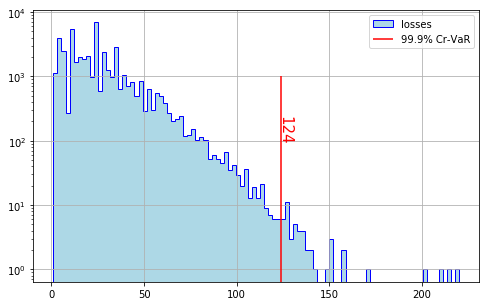
\includegraphics[width=0.7\textwidth]{figures/credit_metrics.png}
	\caption{Distribution of the losses estimated from simulation of credit rating changes within 1 year. The red line shows the 99.9\% Cr-VaR.}
\end{figure}

\section{Credit Valuation
Adjustment}\label{credit-valuation-adjustment}

Suppose you have a portfolio of derivatives with a counter-party. 
If the counter-party defaults and the present value of the portfolio at
default is positive to the surviving party, then the surviving party only
gets a recovery fraction of the portfolio value from the defaulted entity. If however the present value is negative to the surviving party,
it has to pay it in full to the liquidators of the defaulted entity. This creates and asymmetry that, once one has done all
calculations, says that the value of the deal under counter-party risk is
the value without counter-party risk minus a positive adjustment, called
Credit Valuation Adjustment (CVA).

%Therefore we charge the default risky one
%a supplementary amount besides the default-free cost of the contract.
%This is often called Credit Valuation Adjustment, or CVA. 

It can be expressed in the following way:

\begin{equation}
\text{CVA} = (1-R) \int_0^T D(t) \cdot EE(t) d\mathbb{P}(t)
\label{eq:cva}
\end{equation}

where \(T\) is the latest maturity in the portfolio, \(D\) is the
discount factor, \(EE\) is the expected exposure or
\(\mathbb{E}[\text{max(0, NPV}_\text{portfolio})]\).

For an easier computation it is natural to discretize the above integral
and use a time grid going from 0 to the maturity of the portfolio:

\begin{equation}
\text{CVA} = (1-R) \sum_i^n D(t_i) \cdot EE(t_i) \mathbb{P}(t_{i-1}, t_i)
\label{eq:cva_discrete}
\end{equation}

Let us say that Credit VaR measures the risk of losses you
face due to the possible default of some counter-parties you are having
business with. CVA measures the pricing component of this risk, i.e.
the adjustment to the price of a product due to this risk.

\subsection{Debit Valuation Adjustment}

The adjustment seen from the point of view of our counter-party is positive, and is called Debit Valuation Adjustment, DVA. It is positive because the early default of the client itself would imply a discount on the client payment obligations, and this means a gain in a way. So the client marks a positive adjustment over the risk free price by adding the positive amount called DVA. 

Basically when both parties have the possibility to default, they
consistently include both defaults into the valuation. Hence
every party needs to include its own default besides the default of the
counter-party into the valuation. So they will mark a positive
CVA to be subtracted and a positive DVA to be added to the default
risk free price of the deal. The CVA of one party will be the DVA of
the other one and viceversa.

\[
\textrm{price}=\textrm{default risk free price + DVA - CVA}
\]
Now, since
\[
\textrm{default risk free price(A)} = - \textrm{default risk free price(A)}
\]
\[
\textrm{DVA(A)} = \textrm{CVA(B)}
\]
\[
\textrm{DVA(B)} = \textrm{CVA(A)}
\]
we get that eventually
\[
\textrm{price(A)} = -\textrm{price(B)}
\]
so that both parties agree on the price, or, we could say, there is money
conservation.

\subsection{CVA Computation}

The computation of the CVA is easily carried on with Monte Carlo simulation.
First simulate the development of your derivatives portfolio (its NPC) at each time point for each MC scenario. 
Then calculate the CVA using Eq.~\ref{eq:cva} or its discrete form of Eq.~\ref{eq:cva_discrete}.
Finally average the CVA of all the scenarios to get its best estimate.





